\documentclass[12pt]{beamer}
\usepackage{minted}
\usepackage[english, russian]{babel}
\usepackage[utf8]{inputenc}
\usepackage{graphicx}
\usepackage{hyperref}

\hypersetup{
    colorlinks=true,
    linkcolor=blue,
    filecolor=magenta,      
    urlcolor=cyan,
    pdftitle={Overleaf Example},
    pdfpagemode=FullScreen,
    }
\graphicspath{ {./assets/} }
\usetheme{Madrid}

\title{Material Design}
\author{Karabalin Ruslan}
\date{\today}

\begin{document}
	
	\begin{frame}
		\titlepage
	\end{frame}
	
	\begin{frame}
		\frametitle{What is Material?}
		
		\href{https://m3.material.io/}{Material Design} - это система дизайна,
        созданная и поддерживаемая дизайнерами и разработчиками Google.
        Material.io включает в себя подробное руководство по UX
        и реализацию компонентов пользовательского интерфейса
        для Android, Flutter и Web. \\
		
		Последняя версия, Material 3,
        обеспечивает персональный, адаптивный
        и выразительный опыт - от динамических цветов
        и расширенной доступности до основ
        для макетов на больших экранах и дизайнерских маркеров.
		
	\end{frame}
	
	\begin{frame}
		\frametitle{Main Goal}

        \begin{columns}
            \begin{column}{0.5\textwidth}
                Создать визуальный язык,
                который синтезирует классические принципы
                xорошего дизайна с инновациями
                и возможностями технологий и науки. \\

                Разработать единую базовую систему,
                обеспечивающую единый опыт работы
                на разных платформахи устройствах.
            \end{column}
            
            \begin{column}{0.5\textwidth}
                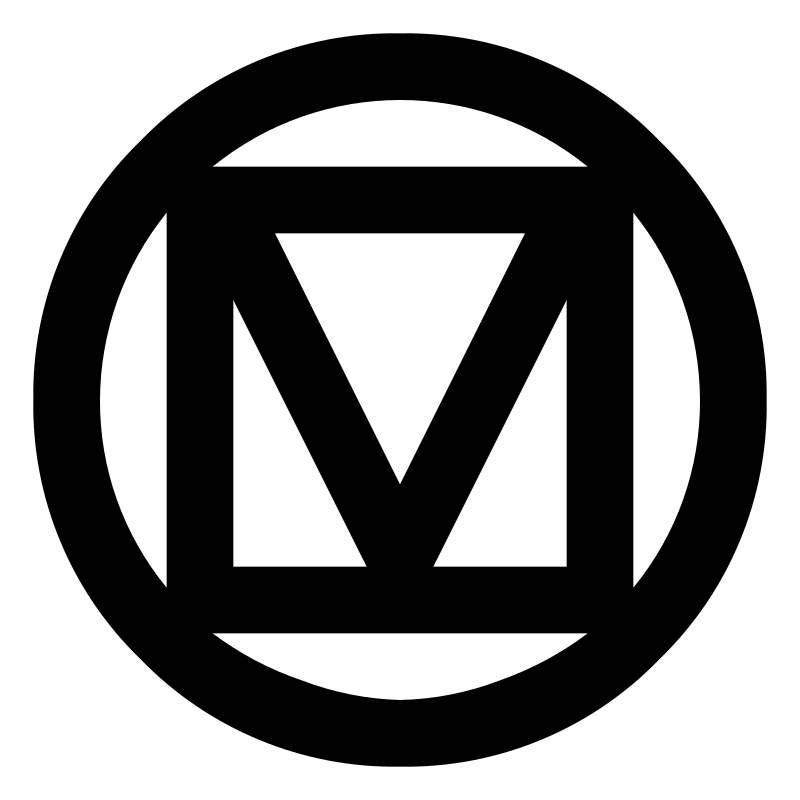
\includegraphics[width=0.8\textwidth]{md.png}
            \end{column}

        \end{columns}

	\end{frame}

    \begin{frame}
        \frametitle{Jetpack Compose}

        \begin{columns}

            \begin{column}{0.5\textwidth}
                
\includegraphics[width=0.8\textwidth]{jc.png}
            \end{column}

            \begin{column}{0.5\textwidth}
                \href{https://developer.android.com/compose}{Jetpack Compose}
                - это современный набор инструментов Android
                для создания нативного пользовательского интерфейса.
                Поддерживается Material Design 3.
            \end{column}

        \end{columns}

    \end{frame}

    \begin{frame}
        \frametitle{Actions}
    
        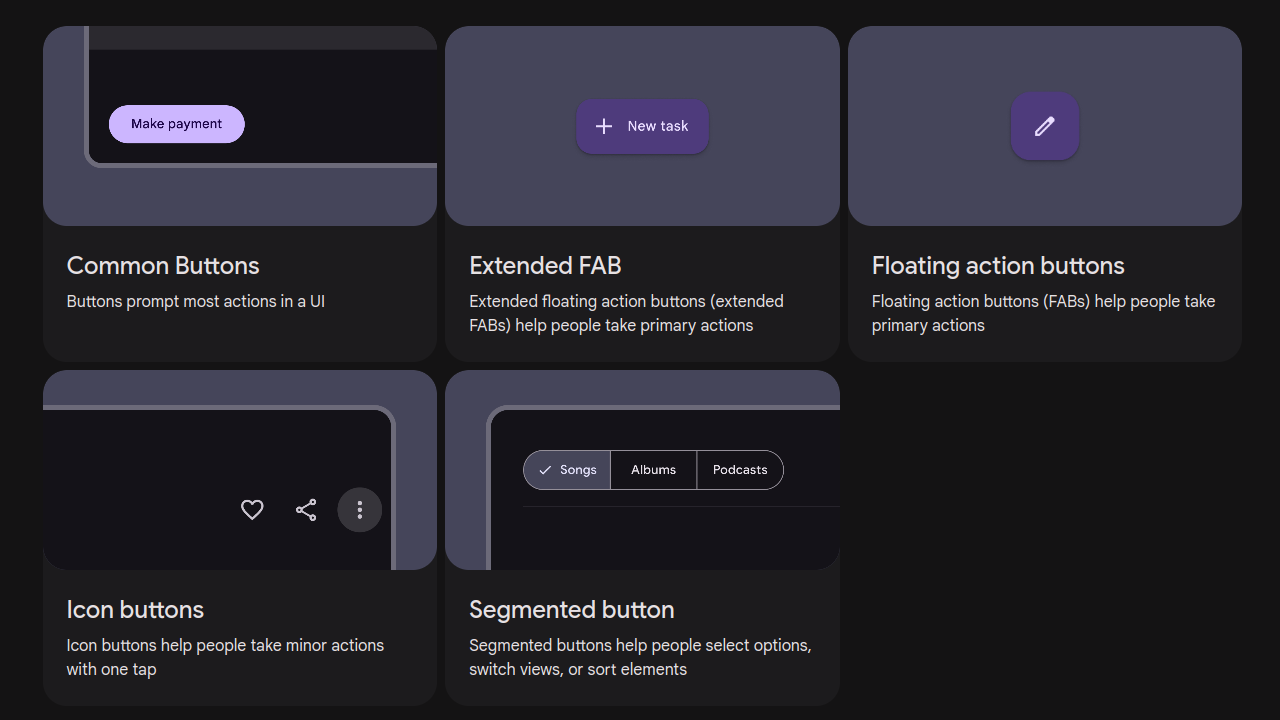
\includegraphics[width=1\textwidth]{actions.png}
    
    \end{frame}

    \begin{frame}
        \frametitle{Communication}
    
        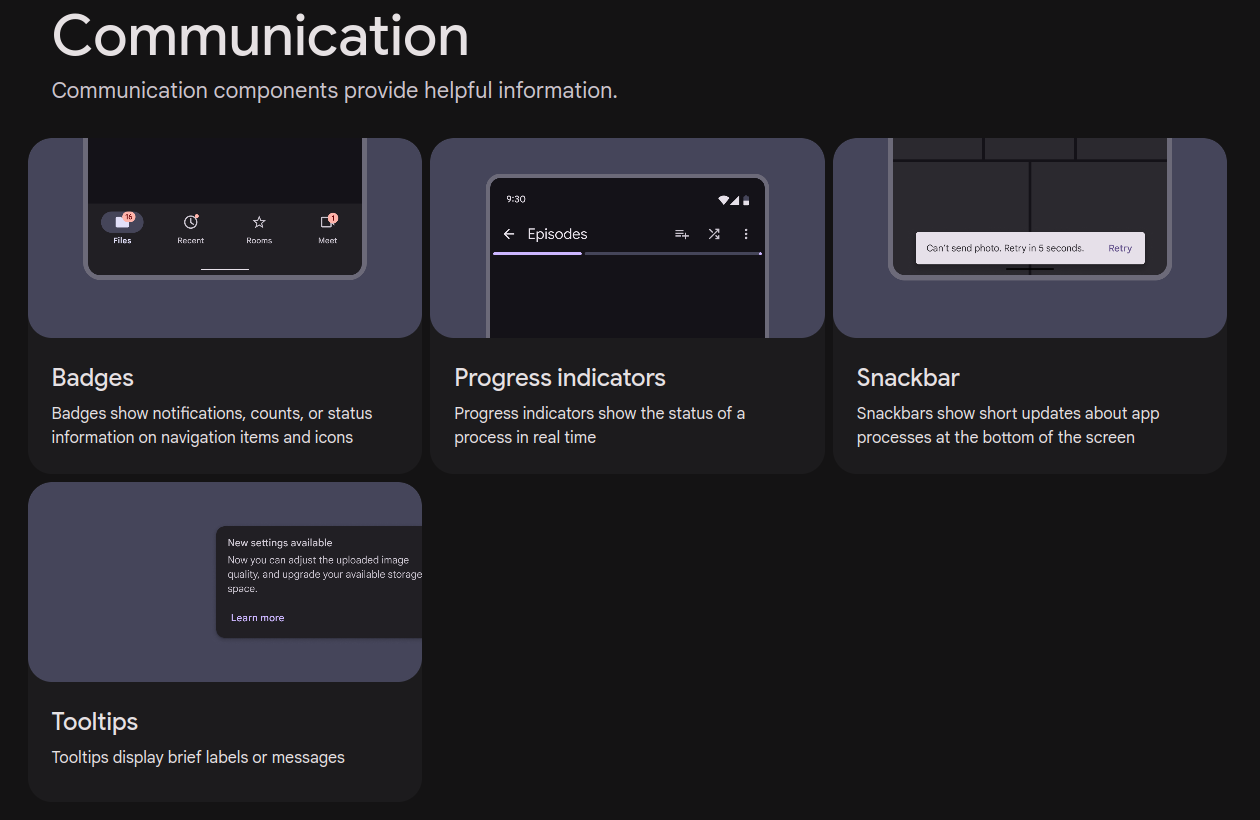
\includegraphics[width=1\textwidth]{communication.png}
    
    \end{frame}

    \begin{frame}
        \frametitle{Containment}
    
        \begin{center}

            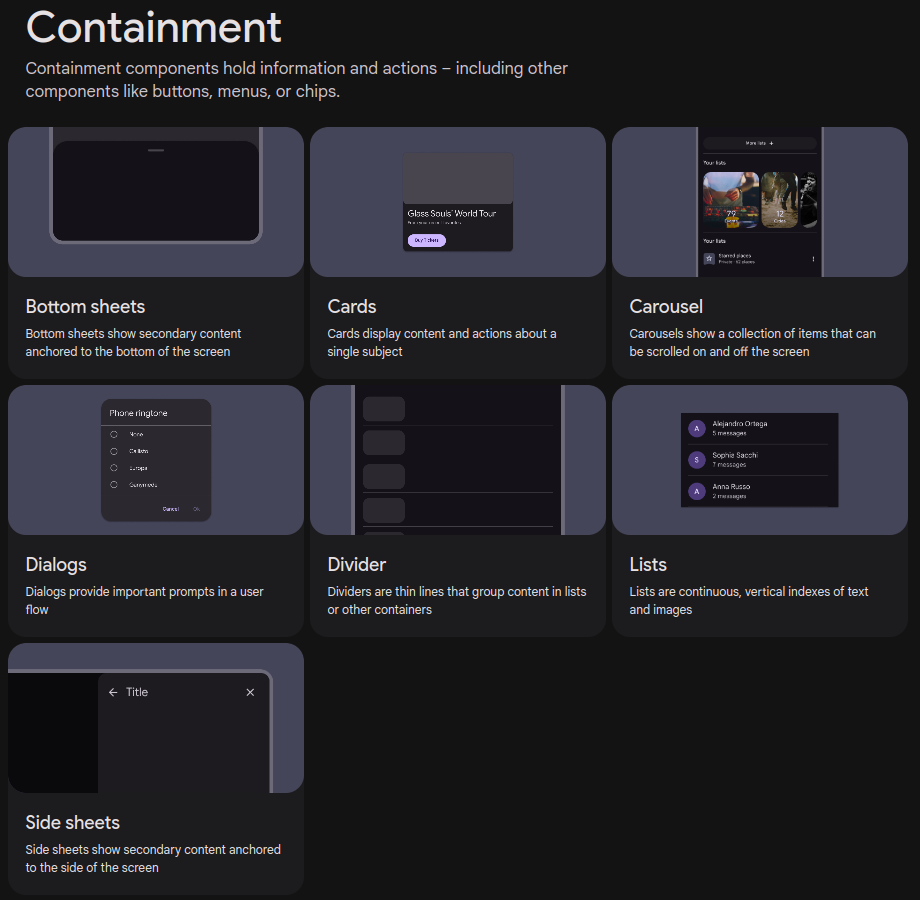
\includegraphics[width=0.65\textwidth]{containment.png}

        \end{center}
    
    \end{frame}

	\begin{frame}
        \frametitle{Navigation}
    
        \begin{center}

            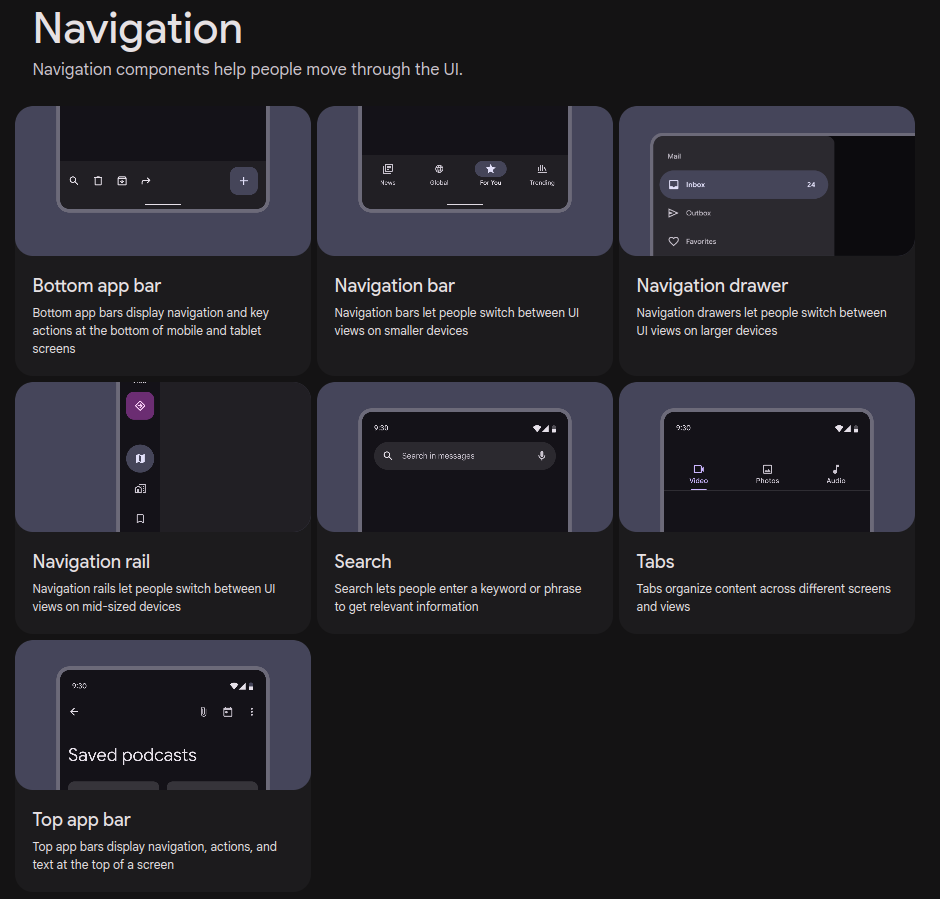
\includegraphics[width=0.65\textwidth]{navigation.png}

        \end{center}
    
    \end{frame}

    \begin{frame}
        \frametitle{Selection}
    
        \begin{center}

            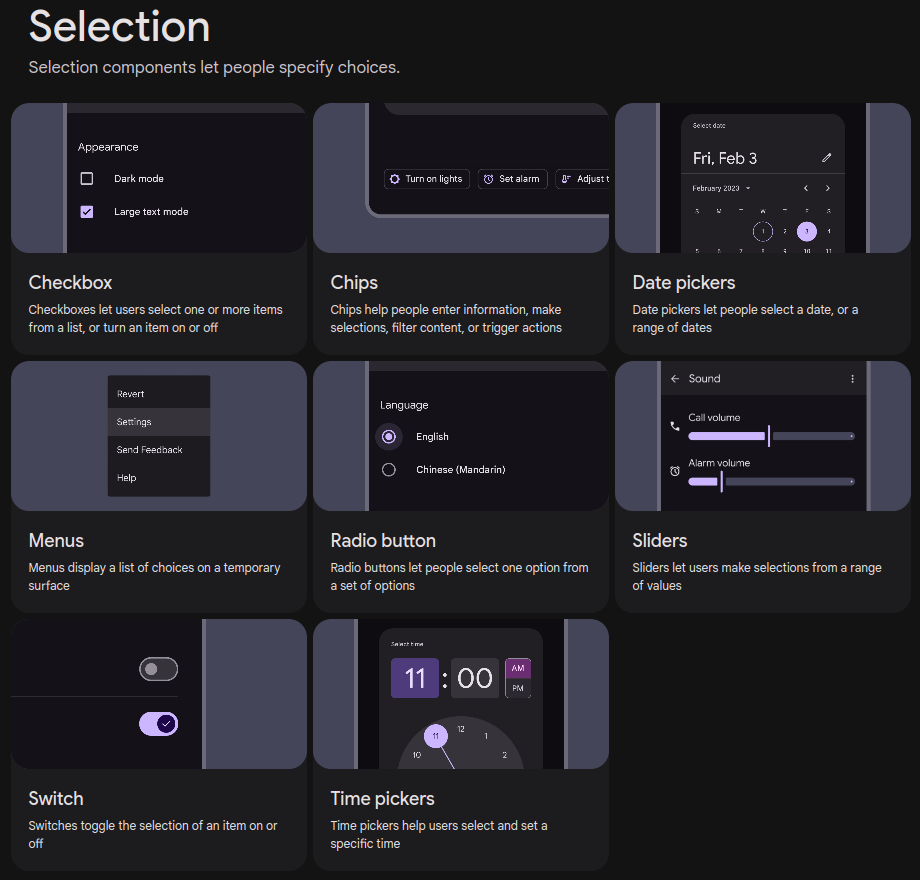
\includegraphics[width=0.65\textwidth]{selection.png}

        \end{center}
    
    \end{frame}

    \begin{frame}
        \frametitle{Text inputs}
    
        \begin{center}
            
            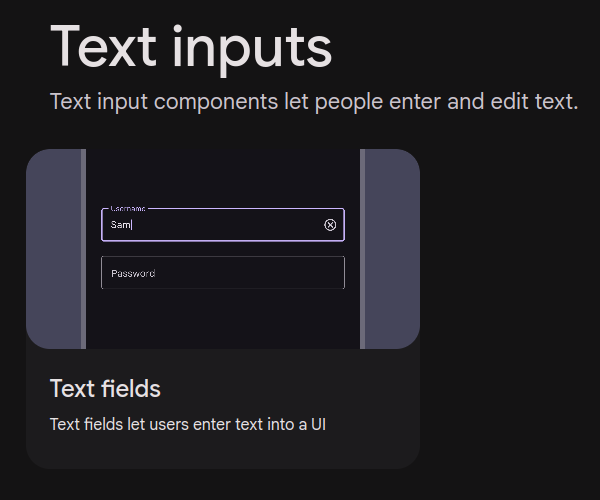
\includegraphics[width=0.5\textwidth]{text-inputs.png}

        \end{center}
    
    \end{frame}

\end{document}
